\documentclass{beamer}

\usepackage{framed}
\usepackage{graphicx}

\begin{document}
%============================================================%
\section{Conditioning on other variables}
\begin{frame}
	\frametitle{Seaborn Workshop}
	\large
\textbf{Conditioning on other variables}
	\begin{itemize}
\item The plots above show many ways to explore the relationship between a pair of variables.
\item Often, however, a more interesting question is “how does the relationship between these two variables change as a function of a third variable?” 
\item This is where the difference between \texttt{regplot()} and \texttt{lmplot()} appears. 
\item While \texttt{regplot()} always shows a single relationsihp, \texttt{lmplot()} combines \texttt{regplot()} with FacetGrid to provide an easy interface to show a linear regression on “faceted” plots that allow you to explore interactions with up to three additional categorical variables.
	\end{itemize}

\end{frame}
%===========================================================%
\begin{frame}[fragile]
	\frametitle{Seaborn Workshop}
\large

The best way to separate out a relationship is to plot both levels on the same axes and to use color to distinguish them:
\begin{verbatim}
sns.lmplot(x="total_bill", y="tip", 
           hue="smoker", data=tips);
\end{verbatim}

\begin{figure}
	\centering
	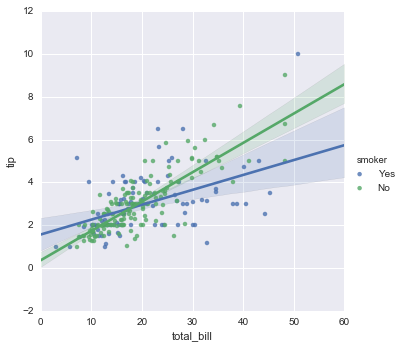
\includegraphics[width=0.55\linewidth]{images/regression_39_0}
\end{figure}
\end{frame}
%===========================================================%
\begin{frame}[fragile]
	\frametitle{Seaborn Workshop}
	\large
	
	In addition to color, it’s possible to use different scatterplot markers to make plots the reproduce to black and white better. You also have full control over the colors used:
\begin{verbatim}
sns.lmplot(x="total_bill", y="tip", hue="smoker", data=tips,
           markers=["o", "x"], palette="Set1");
 \end{verbatim}
\begin{figure}
	\centering
	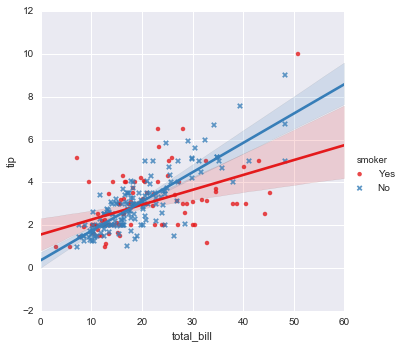
\includegraphics[width=0.7\linewidth]{images/regression_41_0}
\end{figure}
\end{frame}
%==============================================%
\begin{frame}[fragile]
	\large
To add another variable, you can draw multiple “facets” which each level of the variable appearing in the rows or columns of the grid:
\begin{verbatim}
sns.lmplot(x="total_bill", y="tip", 
           hue="smoker", col="time", 
           data=tips);
\end{verbatim}

\begin{figure}
\centering
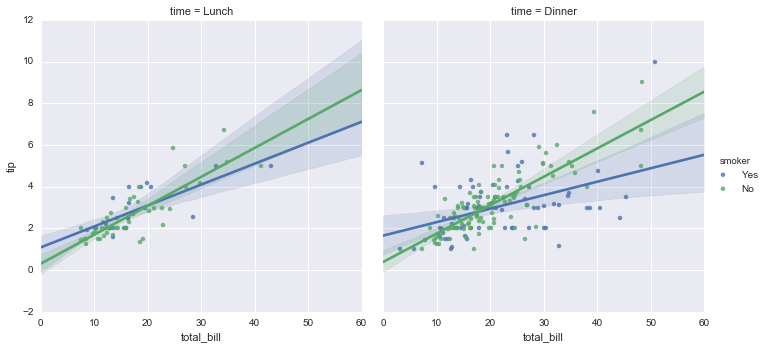
\includegraphics[width=0.55\linewidth]{images/regression_43_0}
\end{figure}

\end{frame}
%===========================================================%
\begin{frame}[fragile]
	\frametitle{Seaborn Workshop}
	\large
\begin{verbatim}
sns.lmplot(x="total_bill", y="tip", hue="smoker",
           col="time", row="sex", data=tips);
\end{verbatim}

\begin{figure}
	\centering
	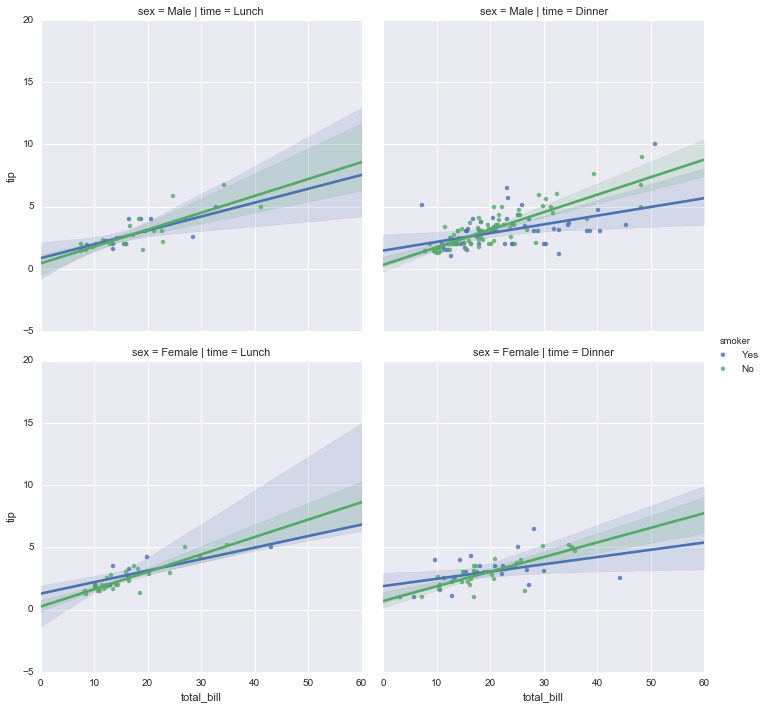
\includegraphics[width=0.7\linewidth]{images/regression_44_0}
\end{figure}
\end{frame}
%=============================================================%
\section{Controlling the size and shape of the plot}
\begin{frame}[fragile]
		\frametitle{Seaborn Workshop}
		\large
	\begin{itemize}
\item Before we noted that the default plots made by \texttt{regplot()} and \texttt{lmplot()} look the same but on axes that have a different size and shape. This is because func:regplot is an “axes-level” function draws onto a specific axes.
\item  This means that you can make mutli-panel figures yourself and control exactly where the the regression plot goes. 
\item If no axes is provided, it simply uses the “\textit{currently active}” axes, which is why the default plot has the same size and shape as most other matplotlib functions. To control the size, you need to create a figure object yourself.
	\end{itemize}

\end{frame}
%=========================================%
\begin{frame}[fragile]
		\frametitle{Seaborn Workshop}
		\large
\begin{framed}
\begin{verbatim}
f, ax = plt.subplots(figsize=(5, 6))
sns.regplot(x="total_bill", y="tip", 
            data=tips, ax=ax);
\end{verbatim}
\end{framed}
\begin{figure}
	\centering
	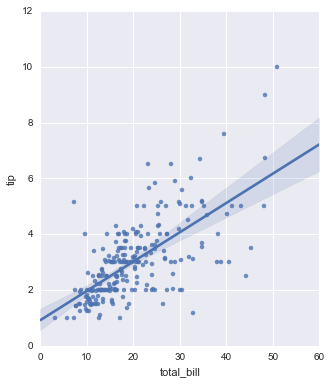
\includegraphics[width=0.55\linewidth]{images/regression_46_0}
\end{figure}
\end{frame}
%===========================================================%
\begin{frame}[fragile]
	\frametitle{Seaborn Workshop}
	\large
	\begin{itemize}
\item In contrast, the size and shape of the \texttt{lmplot()} figure is controlled through the \texttt{FacetGrid} interface using the size and aspect parameters, which apply to each facet in the plot, not to the overall figure itself:
	\end{itemize}

\end{frame}
%===========================================================%
\begin{frame}[fragile]
	\frametitle{Seaborn Workshop}
	\large
	\begin{verbatim}
sns.lmplot(x="total_bill", y="tip", col="day", data=tips,
col_wrap=2, size=3);
	\end{verbatim}

\begin{figure}
	\centering
	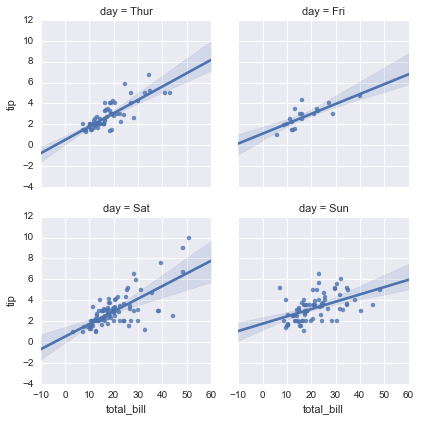
\includegraphics[width=0.55\linewidth]{images/regression_48_0}
\end{figure}
\end{frame}
%===========================================================%
\begin{frame}[fragile]
	\frametitle{Seaborn Workshop}
	\large
\begin{verbatim}
	sns.lmplot(x="total_bill", y="tip", col="day", data=tips,
	aspect=.5);
\end{verbatim}

\begin{figure}
	\centering
	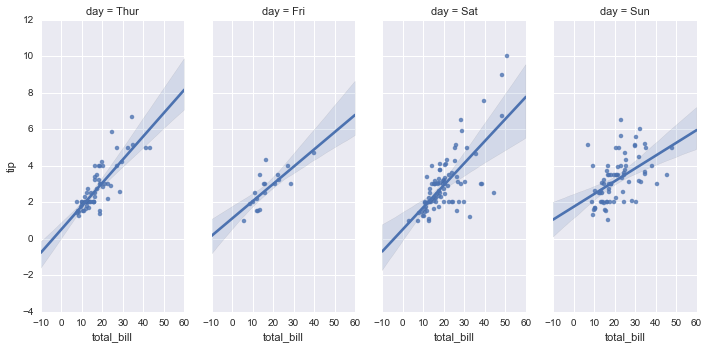
\includegraphics[width=0.7\linewidth]{images/regression_49_0}
\end{figure}
%============================================================%
\end{frame}
\end{document}
